%----------------------------------------------------------------------------------------
%	PACKAGES AND DOCUMENT CONFIGURATIONS
%----------------------------------------------------------------------------------------

\documentclass[
	a4paper, % Paper size, specify a4paper (A4) or letterpaper (US letter)
	10pt, % Default font size, specify 10pt, 11pt or 12pt
]{report}

\usepackage[utf8]{inputenc} % UTF-8 encoding
\usepackage[english]{babel} % Document language - required for customizing section titles
\usepackage{hyperref} % For hyperlinks
\hypersetup{
    colorlinks=true,
    linkcolor=black,
}

\usepackage{geometry}
\geometry{top=3cm} % Adjust the top margin as needed
\geometry{bottom=2.8cm} % Adjust the bottom margin as needed

\usepackage{graphicx} % Required for the inclusion of images

\usepackage{caption} % Required for the inclusion of captions
\captionsetup{format=plain} % Removes any additional formatting after caption

\usepackage{float} % Allows putting an [H] in \begin{figure} to specify the exact location of the figure
\usepackage{booktabs} % Required for better horizontal rules in tables

\usepackage{amsmath, amssymb, amsthm} % Required for some math elements
\usepackage{siunitx} % Required for alignment of numbers with units

\usepackage{titlesec} % For custom section numbering format
\renewcommand{\thesection}{\arabic{section}} % Custom section numbering format (without prefix)

\usepackage[autostyle]{csquotes} % Required for block quotes

% \usepackage{biblatex} % Required for bibliography management
% \addbibresource{main.bib} % Bibliography file (located in the same folder as the main)


%----------------------------------------------------------------------------------------

\begin{document}

	%----------------------------------------------------------------------------------------
	%	REPORT INFORMATION
	%----------------------------------------------------------------------------------------

	\begin{titlepage}
		\centering
		\vspace{1.5cm} % Adjust vertical space

			
\includegraphics[width=1\textwidth]{figures/unimi.jpg} % University logo

		\vspace{1.5cm}
			
			\Huge Lab Report:\\ Logic Gates % Report title
			
		\vspace{1cm}
			
			\Large Lorenzo \textsc{Liuzzo} % Author name(s), add additional authors like: '\& James \textsc{Smith}'
			
		\vspace{2cm}
		
			\begin{tabular}{l r}
			
				Bachelor's Degree: & Physics \\ % Degree
				Course: & Electronics Laboratory \\ % Course
				Academic Year: & 2022/2023 \\ % Accademic year
				\\
				Instructor: & Professor Valentino \textsc{Liberali} \\ % Instructor/supervisor
				Partners: & Jiahao \textsc{Miao} \\ & Riccardo \textsc{Salto} \\ % Partner names
				\\
				Date Performed: & May 24, 2023 \\ % Date the experiment was performed
				
			\end{tabular}

		\vfill % Fill the rest of the page with whitespace
	\end{titlepage}


	%----------------------------------------------------------------------------------------
	%	ABSTRACT & TOC
	%----------------------------------------------------------------------------------------

		\abstract
In the realm of electronics and signal processing, a profound understanding of circuit behavior is paramount for designing high-efficiency systems. 
The primary objective of this experiment was to delve into the intricacies of differentiator and integrator circuits, shedding light on their frequency responses.
To achieve this, custom-tailored circuits were meticulously constructed to fulfill the distinct roles of measuring rate of change and cumulative input. 
Through comprehensive frequency sweeps that encompassed a spectrum from low to high frequencies, intricate data regarding gain and phase behaviors were collected and systematically scrutinized, 
revealing distinct patterns and behaviors across different frequency ranges. 

		{\let\clearpage\relax \tableofcontents}
		

	%----------------------------------------------------------------------------------------
	%	SECTIONS
	%----------------------------------------------------------------------------------------
		
		\clearpage % Forces the first chapter to start on an odd page so it's on the right

		\section{Introduction}
    %%% some intro stuff

    \subsection{Resistor-Transistor Logic}
        Resistor-Transistor Logic (RTL) is a fundamental digital logic family extensively used in electronic circuit design. 
        It leverages transistors for logic gates and integrates resistors for biasing and signal conditioning. 
        This straightforward and cost-effective approach to building digital circuits lays the groundwork for advanced logic families and integrated circuits. 

    \subsection{Bipolar Junction Transistor}
        The Bipolar Junction Transistor (BJT) is comprised of three layers: the emitter, the base, and the collector. 
        N-type and P-type materials, each doped with different impurities, compose these layers. 
        The emitter and collector are doped oppositely, either with excess electrons or holes, while the base remains lightly doped. 
        This setup creates two types of BJTs: NPN and PNP, defined by the arrangement of the layers.
        \begin{figure}[H]
            \centering
            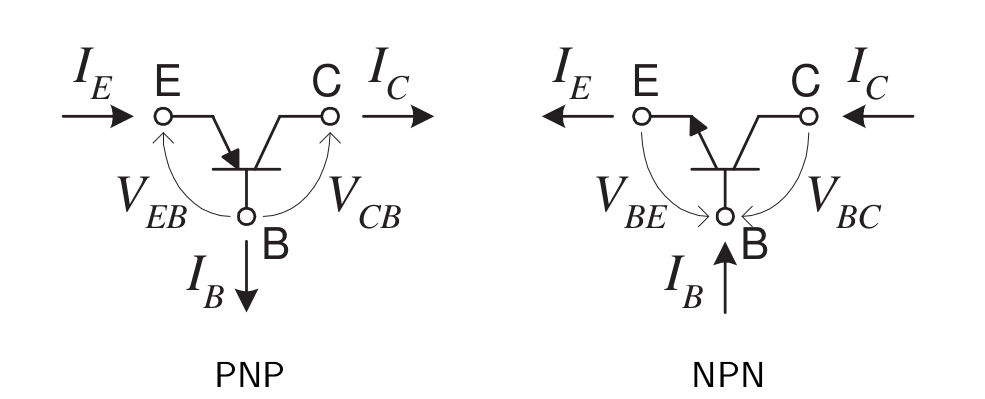
\includegraphics[width=0.7\textwidth]{figures/PNP_NPN.png}
            \caption{PNP and NPN Bipolar Junction Transistors}
            \label{fig:PNP_NPN}
        \end{figure}
        \noindent
        In its off state, the BJT functions as a switch, effectively isolating the collector from the emitter. 
        This behavior is consistent for both NPN and PNP BJTs. During this state, the collector-emitter junction acts as a barrier, preventing any significant current flow, much like a dam restraining water. 
        Additionally, the base-emitter junction remains non-conductive, blocking the flow of current from the emitter to the collector. \\
        Transitioning to the active state, the BJT takes on the role of a signal amplifier. A small current flows from the emitter to the base, giving rise to a more substantial current that courses from the collector to the emitter. 
        This relationship between the base and collector currents forms the cornerstone of the BJT's amplification capability. \\\\
        This amplification phenomenon hinges on the controlled movement of charge carriers across the emitter-base junction. 
        As electrons (or holes) traverse this junction, they engage with the majority carriers in the adjacent layer, resulting in the creation of localized charge regions. 
        These regions facilitate the flow of current from the collector to the emitter. \\
        In the NPN BJT, electrons cross from the emitter to the base. 
        The thinness of the base region and the attractive force exerted by the positively doped collector allow some electrons to overcome the barrier and reach the collector. 
        The modest base current exerts a substantial influence, enabling small variations in its magnitude to produce significant changes in the collector current. \\
        Similarly, the PNP BJT witnesses the flow of holes from the emitter to the base, and the base current governs the larger collector current. 
        In this configuration, the base-emitter junction, now comprised of N-type emitter material and P-type base material, emulates the behavior exhibited by the NPN counterpart. 
        Holes traverse the base region, ultimately converging at the collector, thus amplifying the overall current. \\\\
        As we increase the base current, a point is reached where the collector current can't increase further, regardless of the base current's rise. 
        This state is called saturation. It's as if the BJT switch is turned on fully, allowing maximal current flow through the collector-emitter path. \\
        On the opposite side, as the base current drops, the collector current also decreases until it nearly vanishes. 
        This state is known as cutoff, where the BJT operates as a near-perfect insulator, stopping any significant current from flowing through the collector-emitter junction.
        
    \subsection{Boolean Algebra}        
    
		
		\section{Basic Logic Gates}
			There are three basic logic gates from which any Boolean circuit may be built up. 
			Any function in binary mathematics may be implemented using only the logic gates NOT, AND, and OR.
			\subsection{NOT}
    The NOT gate, also known as an inverter, is the simplest type of logic gate. 
    The circuitry consists of a single transistor along with some associated resistors, as shown in Figure \ref{fig:NOT_circuit}. \\
    It is equivalent to the logical negation operator ($\neg$) in mathematical logic, as its primary function is to output the logical complement of the input.
    Its operation can be algebraically represented as $\text{NOT}(A) = \overline{A}$, while its analytical representation is $f(A)=1-A$, where $A$ is the input signal. \\
    When the input is high (1), the transistor is turned on, creating a low output (0). 
    Conversely, when the input is low (0), the transistor is off, resulting in a high output (1).
    This behavior is consistent with the NOT gate's truth table shown in Table \ref{tab:NOT_table}. \\
    The symbol for the NOT gate, in Figure \ref{fig:NOT_sym}, consists of a triangle with a circle at its output.

    \begin{figure}[H]
        \begin{minipage}{0.5\textwidth}
            \centering
            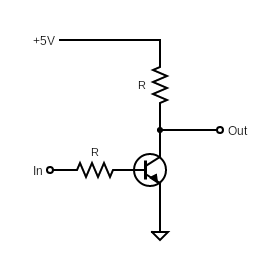
\includegraphics[width=0.8\textwidth]{figures/circuits/NOT.png}
            \captionof{figure}{NOT schematic circuit.}
            \label{fig:NOT_circuit} 
        \end{minipage}
        \begin{minipage}{0.5\textwidth}
            \centering
            \captionof{table}{NOT truth table.}
            \begin{tabular}{|c|c|}
                \hline
                Input & Output \\
                \hline
                0 & 1 \\
                1 & 0 \\
                \hline
            \end{tabular}
            \label{tab:NOT_table}
        \end{minipage}
    \end{figure}

    \begin{figure}[H]
	    \centering
	    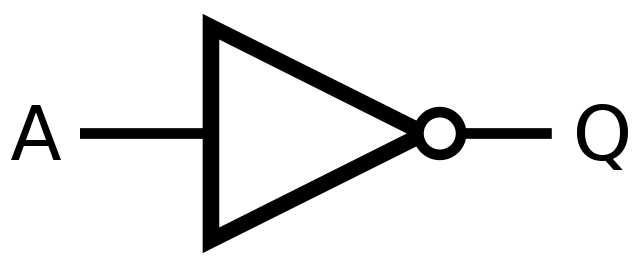
\includegraphics[width=0.3\textwidth]{figures/symbols/NOT.png}
	    \caption{NOT symbol.}
	    \label{fig:NOT_sym} 
	\end{figure}

    % \vspace{1.2cm}
			\subsection{AND}
	The AND gate implements logical conjunction ($\land$) from mathematical logic.
	Its operation can be represented as $\text{AND}(A, B) = A \cdot B$, where $A$ and $B$ are the input signals. \\
	The circuitry of an AND gate involves multiple transistors arranged in series. 
	For a two-input AND gate, two transistors are connected in series, as shown in Figure \ref{fig:AND_circuit}. \\
	If both inputs are high (1), both transistors conduct, creating a low-resistance path from the power supply to the output, resulting in a high output (1). 
	If either or both inputs are low (0), at least one of the transistors will be off, and the output will be pulled to a low state (0). 
    This behavior is consistent with the AND gate's truth table shown in Table \ref{tab:AND_table}. \\
	The symbol for the AND gate is shown in Figure \ref{fig:AND_sym}.

	\begin{figure}[H]
		\begin{minipage}{0.5\textwidth}
			\centering
			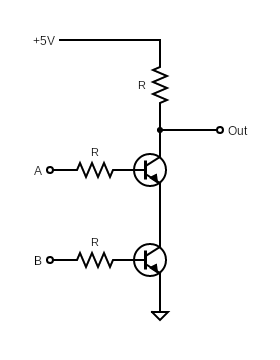
\includegraphics[width=0.8\textwidth]{figures/circuits/AND.png}
			\captionof{figure}{AND schematic circuit.}
			\label{fig:AND_circuit} 
		\end{minipage}
		\begin{minipage}{0.5\textwidth}
			\centering
			\captionof{table}{AND truth table.}
			\begin{tabular}{|c|c|c|}
				\hline
				Input A & Input B & Output \\
				\hline
				0 & 0 & 0 \\
				0 & 1 & 0 \\
				1 & 0 & 0 \\
				1 & 1 & 1 \\
				\hline
			\end{tabular}
			\label{tab:AND_table}
		\end{minipage}
	\end{figure}

	\begin{figure}[H]
	    \centering
	    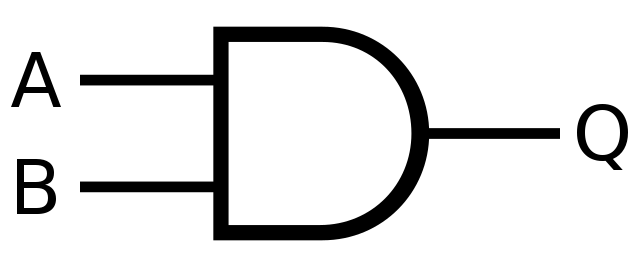
\includegraphics[width=0.3\textwidth]{figures/symbols/AND.png}
	    \caption{AND symbol.}
	    \label{fig:AND_sym} 
	\end{figure}
			\subsection{OR}
    The OR gate represents the logical disjunction ($\lor$) from mathematical logic, and its operation can be represented as $\text{OR}(A, B) = A + B$, where $A$ and $B$ are the input signals. \\
    The circuitry of an OR gate involves multiple transistors arranged in parallel. 
    For a two-input OR gate, two transistors are connected in parallel, as shown in Figure \ref{fig:OR_circuit}. \\
    If either or both inputs are high (1), at least one of the transistors conducts, providing a low-resistance path from the power supply to the output, resulting in a high output (1). 
    Only when both inputs are low (0) will both transistors be off, causing the output to be pulled to a low state (0).
    This behavior is consistent with the OR gate's truth table shown in Table \ref{tab:OR_table}. \\
    The symbol for the OR gate is shown in Figure \ref{fig:OR_sym}.

    \begin{figure}[H]
	    \centering
	    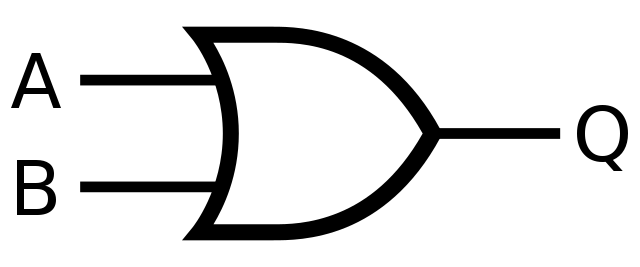
\includegraphics[width=0.3\textwidth]{figures/symbols/OR.png}
	    \caption{OR symbol.}
	    \label{fig:OR_sym} 
	\end{figure}

    \begin{figure}[H]   
        \begin{minipage}{0.5\textwidth}
            \centering
            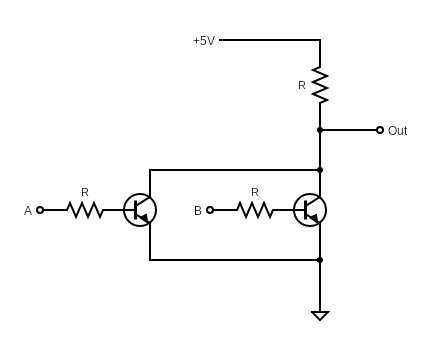
\includegraphics[width=1.1\textwidth]{figures/circuits/OR.png}
            \captionof{figure}{OR schematic circuit.} 
            \label{fig:OR_circuit} 
        \end{minipage}
        \begin{minipage}{0.5\textwidth}
            \centering
            \captionof{table}{OR truth table.}
            \begin{tabular}{|c|c|c|}
                \hline
                Input A & Input B & Output \\
                \hline
                0 & 0 & 0 \\
                0 & 1 & 1 \\
                1 & 0 & 1 \\
                1 & 1 & 1 \\
                \hline
            \end{tabular}
            \label{tab:OR_table}
        \end{minipage}
	\end{figure}

		\newpage
		\section{Universal Logic Gates}
			\section{NAND}
	\begin{figure}[H]
	    \centering
	    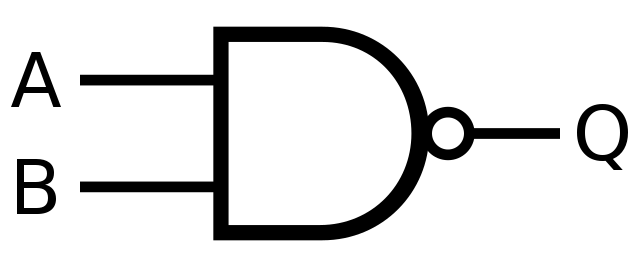
\includegraphics[width=0.3\textwidth]{figures/symbols/NAND.png}
	    \caption{NAND symbol.}
	    \label{fig:NAND_sym} 
	\end{figure}

    \begin{table}[ht]
    \centering
    \begin{tabular}{|c|c|c|}
        \hline
        Input A & Input B & Output \\
        \hline
        0 & 0 & 1 \\
        0 & 1 & 1 \\
        1 & 0 & 1 \\
        1 & 1 & 0 \\
        \hline
    \end{tabular}
    \caption{Truth table for the NAND gate.}
    \end{table}
			\subsection{NOR}
    The NOR gate, short for NOT-OR, can be obtained by connecting an OR gate and a NOT gate in series, as shown in Figure \ref{fig:NOR_gate}. \\
    Its operation can be algebraically represented as $\text{NOR}(A, B) = \overline{A + B}$, where $A$ and $B$ are the input signals.
    When all inputs are low (0), all the transistors in the OR part are off, resulting in a low output (0) for the OR operation. 
    The NOT gate then inverts this low output to a high final output (1).
    This behavior is consistent with the NOR gate's truth table shown in Table \ref{tab:NOR_table}. \\
    The symbol for the NOR gate is shown in Figure \ref{fig:NOR_sym}.

    \begin{figure}[H]   
        \begin{minipage}{0.5\textwidth}
            \centering
            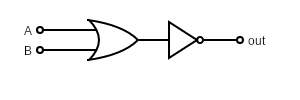
\includegraphics[width=1.1\textwidth]{figures/circuits/NOR.png}
            \captionof{figure}{NOR gate.} 
            \label{fig:NOR_gate} 
        \end{minipage}
        \begin{minipage}{0.5\textwidth}
            \centering
            \captionof{table}{NOR truth table.}
            \begin{tabular}{|c|c|c|}
                \hline
                Input A & Input B & Output \\
                \hline
                0 & 0 & 1 \\
                0 & 1 & 0 \\
                1 & 0 & 0 \\
                1 & 1 & 0 \\
                \hline
            \end{tabular}
            \label{tab:NOR_table}
        \end{minipage}
	\end{figure}

	\begin{figure}[H]
	    \centering
	    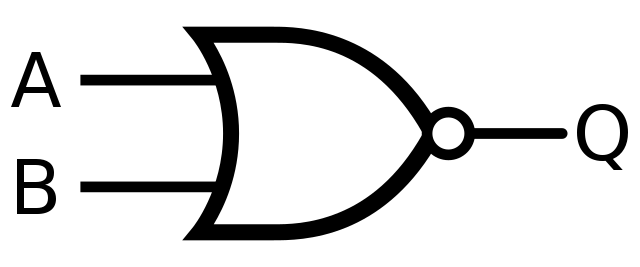
\includegraphics[width=0.3\textwidth]{figures/symbols/NOR.png}
	    \caption{NOR symbol.}
	    \label{fig:NOR_sym} 
	\end{figure}

			
\subsection{Basic Logic Gates form NAND and NOR}
    Both NAND and NOR gates are considered \enquote{universal gates}. 
    This means that any logical function can be constructed using either NAND logic or NOR logic alone. 
    In other words, complex circuits and logical operations can be built using only one type of gate. \\\\
    In this subsection, it is shown how to construct the NOT (Figures \ref{fig:NAND_NOT} and \ref{fig:NOR_NOT}), AND (Figures \ref{fig:NAND_AND} and \ref{fig:NOR_AND}), and OR (Figures \ref{fig:NAND_OR} and \ref{fig:NOR_OR}) gates using only NAND gates and only NOR gates. \\

    \begin{figure}[H]   
        \begin{minipage}{0.5\textwidth}
            \centering
    	    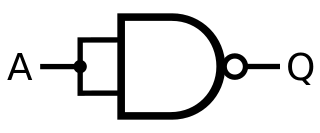
\includegraphics[width=0.6\textwidth]{figures/NOT_from_NAND.png}
	        \caption{NOT gate from a NAND gate.}
	        \label{fig:NAND_NOT} 
	    \end{minipage}	
        \begin{minipage}{0.5\textwidth}
            \centering
    	    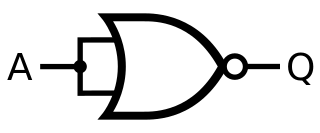
\includegraphics[width=0.6\textwidth]{figures/NOT_from_NOR.png}
            \caption{NOT gate from a NOR gate.}
            \label{fig:NOR_NOT}
        \end{minipage}
    \end{figure}

    \begin{figure}[H]   
        \begin{minipage}{0.5\textwidth}
            \centering
    	    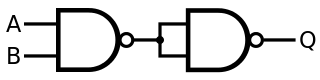
\includegraphics[width=0.8\textwidth]{figures/AND_from_NAND.png}
	        \caption{AND gate from NAND gates.}
	        \label{fig:NAND_AND} 
	    \end{minipage}	
        \begin{minipage}{0.5\textwidth}
            \centering
    	    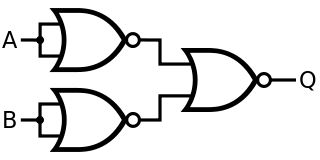
\includegraphics[width=0.6\textwidth]{figures/AND_from_NOR.png}
            \caption{AND gate from NOR gates.}
            \label{fig:NOR_AND}
        \end{minipage}
    \end{figure}

    \begin{figure}[H]   
        \begin{minipage}{0.5\textwidth}
            \centering
    	    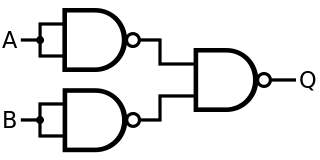
\includegraphics[width=0.6\textwidth]{figures/OR_from_NAND.png}
	        \caption{OR gate from NAND Gates.}
	        \label{fig:NAND_OR} 
	    \end{minipage}	
        \begin{minipage}{0.5\textwidth}
            \centering
    	    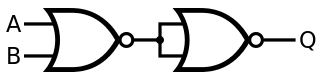
\includegraphics[width=0.8\textwidth]{figures/OR_from_NOR.png}
            \caption{OR gate from NOR Gates.}
            \label{fig:NOR_OR}
        \end{minipage}
    \end{figure}

		\newpage
		\section{Other Logic Gates}
			\section{XOR}
	\begin{figure}[H]
	    \centering
	    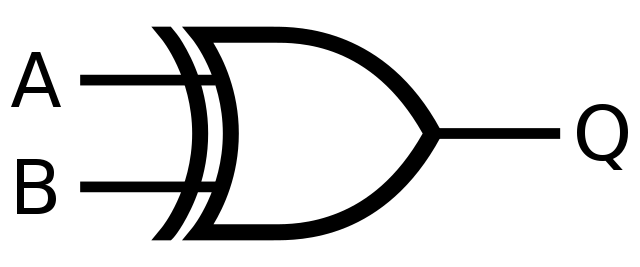
\includegraphics[width=0.3\textwidth]{figures/symbols/XOR.png}
	    \caption{XOR symbol.}
	    \label{fig:XOR_sym} 
	\end{figure}

    \begin{table}[ht]
    \centering
    \begin{tabular}{|c|c|c|}
        \hline
        Input A & Input B & Output \\
        \hline
        0 & 0 & 0 \\
        0 & 1 & 1 \\
        1 & 0 & 1 \\
        1 & 1 & 0 \\
        \hline
    \end{tabular}
    \caption{Truth table for the XOR gate.}
    \end{table}    
		
	%----------------------------------------------------------------------------------------
	%	BIBLIOGRAPHY
	%----------------------------------------------------------------------------------------

		% \printbibliography % Output the bibliography


\end{document}

%----------------------------------------------------------------------------------------
